\chapter{Introduction}
Flow and transport processes between turbulent free-flows and porous-media 
flows are common in a wide range of environmental, industrial, civil and medical 
applications.
For example \textcite{tesi:mosthaf}, \textcite{intro:davarzani} and \textcite  {tesi:fetzer} have studied the effect that a turbulent air flow has on the 
drying rate of an adjacent wet porous-medium, like a soil. This kind of system, 
in spite of its clarity, involves many different physical phenomena that act at 
different scales, thus, because of this complexity, a reliable prediction of 
the evaporation rates is still a challenge. In Figure~\ref{fig:intro} we can 
see a schematic representation of the mechanisms that play a role in such a 
situation, where both transport and thermal effects can be taken into account. 
Moreover, considering natural phenomena, an additional difficulty is given by 
the intrinsic uncertainty and heterogeneity of material properties, such as the 
soil porosity, and atmospheric conditions, such as the air humidity or the 
solar radiation.
\begin{figure}[ht]
	\centering
	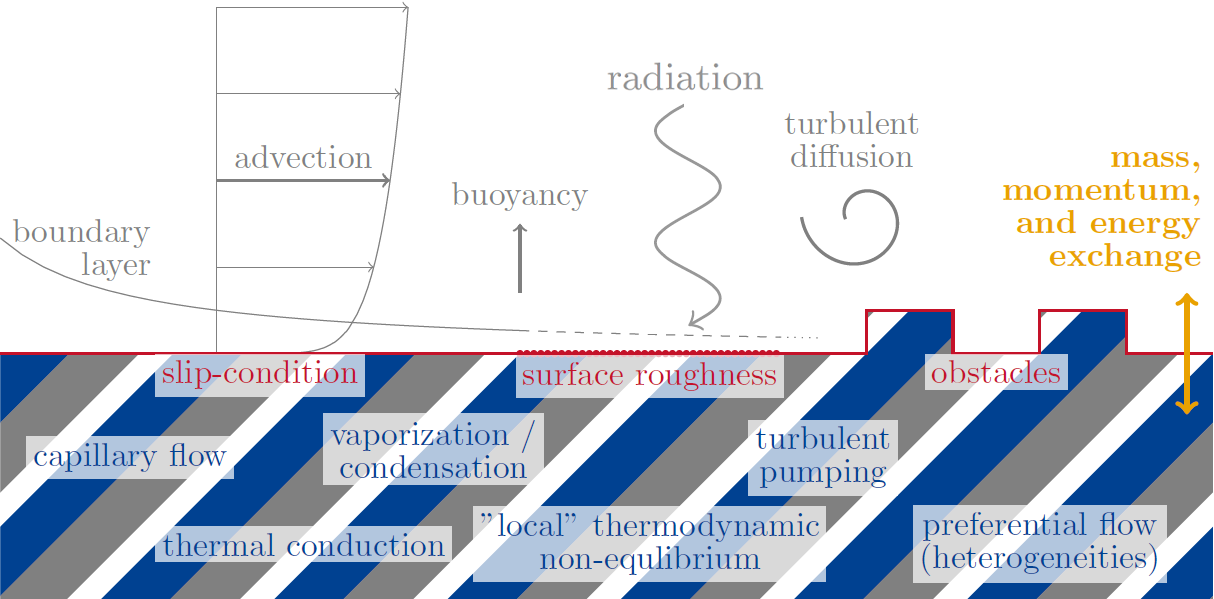
\includegraphics[width=\textwidth]{intropicture2.png}
	\caption[Exchange processes between free and porous-medium 
	flows]{Example of physical phenomena affecting the exchange processes 
		between a free-flow and a porous-medium flow. Figure source: 
		\cite{tesi:fetzer}.}
	\label{fig:intro}
\end{figure}

These studies can be exploited, for example, to better understand the process of soil salinization, that is one of the most serious agricultural problems in many arid and coastal areas in the world. It consists in the excessive accumulation of salt in the soil pores, with the consequence of a partial or complete loss of productivity. A limited amount of salt precipitation in the soil, due to evaporation of irrigation water, is inevitable, but a wrong water management could lead salinity problems in the long term, especially in arid areas where irrigation is necessary to increase the production for food requirements (see \cite{web:fao}). According to \cite{soil:munns}, more than 6\% of wolrd's total land area is salt affected.
The region of the soil near the surface is the most involved in this problem, hence the importance of studying the interactions between the free-flow and the porous-medium flow that there occur. For example, \textcite{intro:salinization} have investigated the application of kinetic approaches to describe the salt precipitation in a coupled system.
\begin{figure}
	\centering
	\subfloat[]{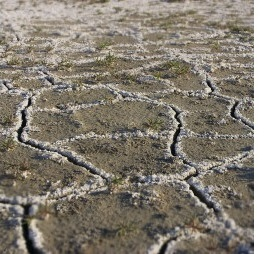
\includegraphics[height=0.22\textheight]{salinity.jpg}}
	\subfloat[]{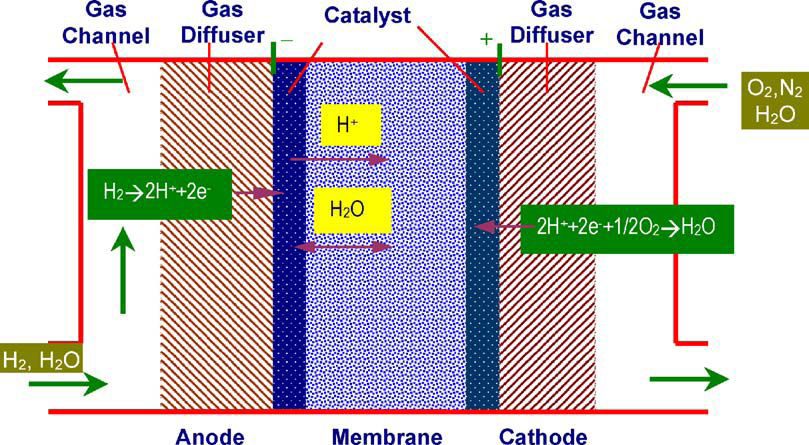
\includegraphics[height=0.22\textheight]{pem.png}}
	\caption{(a): Salt-affected soil. Figure source: \cite{web:fao}. (b): Principle of operation of PEM fuel cells. Figure source: \cite{intro:pemfig}.}
	\label{fig:intro2}
\end{figure}

Switching to a technical framework, PEM (Proton Exchange Membrane) fuel cells represent a possible alternative power source, that could be used for transportations. In their design, transport and diffusion phenomena through gas channels and gas diffusers play an important role in the electrochemical reactions that determine the cell performances and efficiency. As we can see in Figure~\ref{fig:intro2}, reactant gases are supplied at the anode and cathode being transported through gas channels, then they diffuse into porous layers called gas diffusers, that should deliver them uniformly and efficiently to the catalyst layers, where reactions take place (see \cite{wu:fuelcell}, \cite{tesi:baber} and \cite{tesi:pem}). Protons are produced at the anode and transported through the membrane to react with oxygen at the cathode and produce water. The water management within the cells is of great importance because it is essential to have a certain level of humidity in the membrane in order to facilitate the transport of protons, but an excess of water could flood the catalyst layers, with the result of an inhibition of the reactions.
Because of the complex and compact geometry of PEM fuels cells, it is generally difficult and expensive to take measurements, thus mathematical and numerical models are helpful in order to better understand the mechanical, thermal and chemical phenomena that take place to improve the cell performances and lifetime.

In order to study these processes, in the following we focus on the case of the evaporation from 
a porous material and we consider a system that involves two subdomains: the 
upper one with a free-flow and the lower one occupied by a porous-medium, as it is represented in Figure~\ref{fig:intro}.
At the interface between the two subdomains there is exchange of mass, momentum 
and energy.

Numerical studies of this coupled system can be performed with a 
\emph{single-domain} approach or with a \emph{two-domain} approach 
\cite{tesi:fetzer}.

Within the single-domain approach, the same equations are solved in the whole 
computational domain, including both the free-flow region and the 
porous-medium. A first possibility is to use the Navier-Stokes to model the 
flow motion and thus to perform a direct numerical simulation (DNS) of the 
whole system. The porous-medium has to be resolved at the pore-scale, thus a 
detailed knowledge of the pore structure, not easy to obtain for real 
materials, is necessary. The computational effort is very high because 
of the strict spatial and temporal requirements of a DNS and it increases even 
more if the fluid is non-isothermal, multi-phase and multi-component. 
\textcite{intro:dns} and \textcite{intro:dns2} have performed DNS in 
porous-media domains using the lattice Boltzmann method. A cheaper possibility 
for the case of laminar single-phase flows is to employ the Brinkman's equation 
\cite{intro:brinkman}, which is a superposition of the Stokes equations and 
Darcy's law, with a modified viscosity:
\begin{equation}
	-\nabla \cdot (\tilde{\mu} \nabla \mathbf{v}) + \mu 
	\mathbf{K}^{-1}\mathbf{v} + \nabla p = \mathbf{f}.
\end{equation}
Then the transition between the two 
regions can be expressed with a spatial variation of the involved physical 
parameters, either considering a transition region or admitting a discontinuous 
variation at the interface. \textcite{intro:shavit} proposed a modification of 
the Brinkman's equation and applied it to the case of shallow water flows over 
porous surfaces.

Within the two-domain approach, adopted also in this thesis, different set of 
equations are used in the two subdomains and they are coupled imposing suitable 
conditions at the interface.
The free-flow can be described with the Stokes 
equations, Navier-Stokes equations or RANS equations, depending on the flow 
regime. The porous-medium approach instead is usually described with the 
Darcy's law or sometimes with the Forchheimer's law, when the Reynolds number 
is higher.

In \cite{intro:disca2} a single-domain approach (through a penalization) and a 
two-domain approach for 
the Navier-Stokes/Forchheimer coupling are compared, with the results that the 
first is much easier to implement, but the second one describes better the 
physics of the problem. (single-phase, single-component flows).

In \cite{intro:disca} the well posedness for the Stokes/Darcy problem is proved 
and an iterative method for the solution is proposed.

In \cite{tesi:fetzer} several turbulence models are tested and 4 different sets 
of interface conditions for multi-phase, multi component flows are tried. 
Moreover sand-grain roughness is analysed and also obstacles roughness, as in 
our case\\

Consequently a numerical study of this system generally involves a coupled 
model where the free-flow is described by the RANS equations and the 
porous-medium flow is described with a REV-scale approach, such as the Darcy's 
law. 
Simple models for single-phase systems can be generalized to take 
into account multicomponent non-isothermal flows, with one phase in the 
free-flow region and two phases in the porous-medium. Finally the problem 
has to be closed through suitable coupling conditions imposed at the 
interface; they are usually based on phenomenological arguments in order to 
keep the description simple and they should be as close as possible to the 
imposition of thermodynamic the equilibrium~\cite{paper:mosthaf}.

In this thesis the focus is on the improvement of the free-flow model. When the 
flow is in a turbulent regime, turbulent eddies develop near the interface and 
they cascade through consecutively smaller scales until the kinetic energy 
dissipates into internal thermal energy. Because of their location, they have 
a strong influence on the exchange processes between the two subdomains, so an 
accurate evaluation of their behaviour is of crucial importance. Improvements 
can be obtained of course with a refinement of the grid, but also employing 
high order methods; in 
particular, in the discretization of the Navier-Stokes equations using finite 
volumes, a key role is played by the approximation used for the non linear term 
$\nabla \cdot (\mathbf{v} \mathbf{v}^\mathrm{T})$. A common and easy 
choice is to employ a first order upwind approximation for the 
\emph{transported} velocity, but this option can produce solutions with 
excessive numerical diffusion. Other possibilities are given by high order 
methods 
like the Linear Upwind Differencing (LUD) scheme, the Central Differencing (CD) 
scheme or the Quadratic Upstream Interpolation for Convective Kinetics (QUICK) 
scheme; sometimes they can produce 
accurate solution but they have also shown to be unstable in certain 
situations and to produce overshoots or undershoots that 
may lead to unphysical values of quantities that for example have to be 
positive (see \cite{main:vermal}). With this in mind our interest will be in 
the Total Variation Diminishing (TVD) methods, a family of methods that has 
been derived with the purpose of providing a solution with a second order 
accuracy, but without any risk of numerical oscillations. They are called also 
high resolution methods.

In Chapter~\ref{chap:equations} the equations employed in the models will be 
presented, with particular attention to the free-flow equations. In 
Chapter~\ref{chap:discretization} the finite volume method will be described 
and in Subsection~\ref{subsec:tvd} the TVD methods will be introduced. At last, 
in Chapter~\ref{chap:results}, the numerical results will be shown; in 
particular we will see the application of the TVD methods to the Navier-Stokes 
equations in comparison to the first order upwind scheme, then two tests 
involving turbulent flows and finally a more complex scenario involving 
obstacles at the interface between a free-flow region and a porous-medium.

The high order methods mentioned above have been implemented in the framework 
of the open-source simulator \DUMUX: DUNE for multi-$\{$phase, component, 
scale, physics, \dots$\}$ flow in porous-media, see \cite{dumux:tutti} and 
\cite{dumux:flemisch}. \DUMUX is an 
additional module of DUNE (Distributed and Unified Numerics Environment, 
\cite{web:dune}) and, through the use of an object-oriented design in 
conjunction with template programming, it provides a C++ environment that 
allows an efficient implementation of numerical models related to porous-media 
flows.

All the source code used for the simulations performed can be 
found at \url{https://git.iws.uni-stuttgart.de/dumux-pub/vescovini2019a}, 
together with the instructions to install the required software.